\documentclass[]{article}
\usepackage{graphicx}
\usepackage{blindtext}
\usepackage{hyperref}
\graphicspath{ {./images/} }
\usepackage[spanish]{babel}
%opening
\title{Resumen sobre estadística y probabilidad.}
\author{Leandro Molina}

\hypersetup{
	colorlinks=true,
	linkcolor=blue,
	filecolor=magenta,      
	urlcolor=cyan,
	pdftitle={Overleaf Example},
	pdfpagemode=FullScreen,
}

\begin{document}

\maketitle
\vspace{-20pt}

\noindent

\includegraphics[width=\linewidth, height=14cm]{twin_estadistica.png}
%\footnote{Personaje perteneciente a \href{https://www.youtube.com/@TwinSensei}{Twin-Sensei}}
\pagebreak

\tableofcontents


\pagebreak
\section{Capitulo 1. ¿Que es la estadistica?}
\subsection{¿Por qué se debe estudiar estadística?}
Hay 3 motivos para el estudio de la estadística estos son:
\begin{enumerate}
	\item La primera razon, consiste en que la informacion numerica prolifera por todas partes. si revisas diarios o revistas contienen mucha cantidad de informacion numerica.
	\item Una segunda razon, es que las tecnicas de la estadistica se emplean para tomar decisiones que afectan la vida diaria, es decir, que incluyen en su bienestar.
	\item Una tercera razon, el conocimiento de sus metodos facilita la compresion de la forma en que se toman las decisiones y proporciona un entendimiento mas claro de como le afectan. 
\end{enumerate}
Al encarar la necesidad de tomar decisiones en las que tenes que saber hacer un analisis de datos resultara de utilidad. Con el fin de tomar una decision informada, sera necesario llevar a cabo lo siguiente para poder tomar una decision informada:
\begin{enumerate}
	\item Determinar si existe informacion adecuada o si requiere informacion adicional.
	\item Reunir informacion adicional, si se necesita, de manera que no se obtengan resultados erroneos.
	\item Resumir los datos de manera util e informativa.
	\item Analizar la informacion disponible.
	\item Obtener conclusiones y hacer inferencias al mismo tiempo que se evalua el riesgo de tomar una decision incorrecta.
\end{enumerate}
En resumen hay por lo menos tres razones para estudiar estadistica: 1) los datos proliferan por todas partes; 2) las tecnicas estadisticas se emplean en la toma de decisiones que influyen en su vida; 3) sin que importe la carrera que elija, tomara decisiones profesionales que incluyan datos.

\subsection{¿Que se entiende por estadística?}
Posee dos significados: su aceptacion mas comun, la estadistica se refiere a informacion numerica. Una coleccion de informacion numerica recibe el nombre de \textbf{estadisticas}. La informacion estadistica se presenta en forma grafica, es util porque capta la atencion del lector e incluye una gran cantidad de informacion. 
\begin{flushleft}
\textbf{Estadistica:} Ciencia que recoge, organiza, presenta, analiza e interpreta datos con el fin de propiciar una toma de decisiones mas eficaz.
\end{flushleft}
El primer paso en el estudio de un problema consiste en recoger datos revelantes. Estos deben organizarse de alguna forma y, tal vez, representarse en una grafica.
\subsection{Tipos de estadística.}
El estudio de la estadística se divide en dos categorias: la estadística descriptiva y la estadística inferencial.
\subsubsection*{Estadistica descriptiva.}
Es la ciencia que "recoge, organiza, presenta, analiza...datos". Esta parte de la estadistica recibe el nombre de \textbf{estadistica descriptiva}.

\begin{flushleft}
\textbf{Estadistica descriptiva:} Metodos para organizar, resumir y presentar datos de manera informativa.
\end{flushleft}
Se trata de estadistica descriptiva si calcula el crecimiento porcentual de una decada a otra. Sin embargo, no seria de naturaleza descriptiva si utiliza estos para el calcular con esos datos algo futuro.
Una masa de datos desorganizados resulta de poca utilidad. Las tecnicas de la estadistica descriptiva permiten organizar esta clase de atos y darles significado. Los datos se ordenan en una \textbf{distribucion de frecuencia} (mas adelante lo veremos). Se emplean diversas clases de \textbf{graficas} para describir datos.

\subsubsection*{Estadistica inferencial.}
La estadistica inferencial, tambien denominada \textbf{inferencia estadistica}. El principal interes que despierta esta disciplina se relaciona con encontrar algo relacionado con una poblacion a partir de una muestra de ella. Ya que estas son inferencias relacionadas con una poblacion, basadas en datos de la muestra, se trata de estadistica inferencial. Se podria considerar a la estadistica inferencial como la mejor conjetura que es posible obtener del valor de una poblacion sobre la base de la informacion de una muestra.
\begin{flushleft}
	\textbf{Estadistica inferencial: }Metodos que se emplean para determinar una propiedad de una \textbf{poblacion} con base en la informacion de una \textbf{muestra} de ella.
\end{flushleft}
Atencion a las palabras poblacion y muestra en la definicion de estadistica inferencial. Una \textbf{poblacion} puede constar de individuos, tambien puede consistir en objetos. Desde una perspectiva estadistica, una poblacion no siempre que tiene que ver con personas.

\begin{flushleft}
	\textbf{Poblacion: }Conjunto de individuos u objetos de interes o medidas que se obtienen a partir de todos los medios u objetos de interes.
\end{flushleft}
Con el objeto de inferir algo sobre una poblacion, lo comun es que se tome una muestra de ella.
\begin{flushleft}
	\textbf{Muestra: }Porcion o parte de la poblacion de interes.
\end{flushleft}
La toma de muestras para aprender algo sobre una poblacion es de uso frecuente en administracion, agricultura, politica y acciones de gobierno.

\subsection{Tipos de variables.}
Una variable es una característica observable en las unidades estadísticas y tiene, por lo menos, dos valores. \\
Dos tipos basicos de variables: 1)Cualitativas y 2)Cuantitativas, la caracteristica que se estudia es de naturaleza no numerica, recibe el nombre de \textbf{variable cualitativa} o \textbf{atributo}. Cuando los datos son de naturaleza cualitativa, importa la cantidad o proporcion que caen dentro de cada categoria. Los datos cualitativos se resumen en tablas o graficas de barras. Cuando la variable que se estudia aparece en forma numerica, se le denomina \textbf{variable cuantitativa}. Las variables cuantitativas pueden ser discretas o continuas. Las \textbf{variables discretas} adoptan solo ciertos valores y existen vacios entre ellos. Las variables discretas son el resultados de una relacion numerica, las observaciones de una \textbf{variable continua} toman cualquier valor dentro de un intervalo especifico. Por lo general las variables continuas son el resultado de mediciones. \linebreak Resumen de los tipos de variables: \\
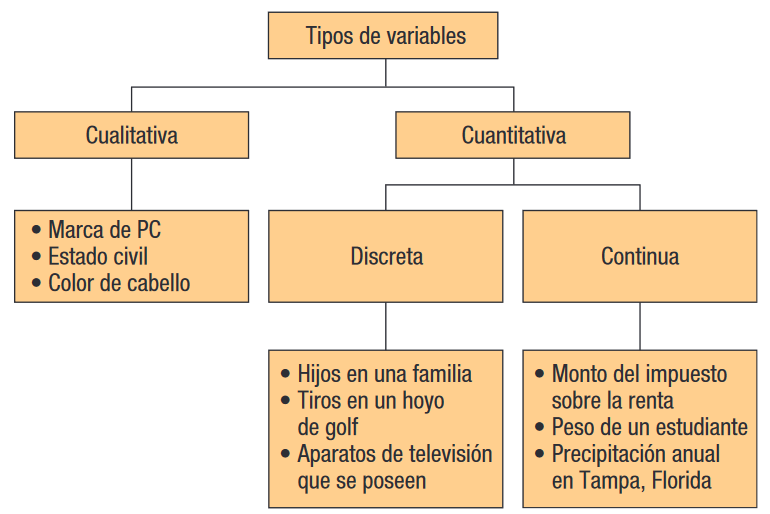
\includegraphics[width=14cm, height=8cm]{resumenTiposVariables1_2}

\subsection{Niveles de medición.}
Los datos se clasifican por niveles de medicion. El nivel de medicion de los datos rige los calculos que se llevan a cabo con el fin de resumir y presentar los datos. Tambien determina las pruebas estadisticas que se deben realizar. De hecho, existen cuatro niveles de medicion: nominal, ordinal, de intervalo y de razon. La medicion mas baja, o mas primaria, corresponde al nivel nominal. La mas alta, o el nivel que proporciona la mayor informacion relacionada con la observacion, es la medicion de razon.

\subsubsection*{Datos de nivel nominal.}
Las observaciones acerca de una variable cualitativa solo se clasifican y se cuentan. No existe una forma particular para ordenar las etiquetas, no existe un orden natural. Para el nivel nominal, la medicion consiste en contar, a veces, para una mejor compresión de lectura, estos conteos se convierten en porcentajes. Es necesario hacer que el porcentaje sume un total de 100\%, no existe un orden natural para los resultados. Para procesar datos a menudo se codifica la informacion en forma numerica. El nivel nominal tiene las siguientes propiedades:
\begin{enumerate}
	\item La variable de interes se divide en categorias o resultados.
	\item No existe un orden natural de los resultados.
	\item Los datos solo se clasifican.
\end{enumerate}

\subsubsection*{Datos de nivel ordinal.}
El nivel inmediato superior de datos es el \textbf{nivel ordinal}. No es posible distinguir la magnitud de las diferencias entre los grupos, ¿la diferencia entre superior y bueno es la misma que entre lo malo e inferior? No es posible afirmarlo. Las propiedades del nivel ordinal de los datos son las siguientes:
\begin{enumerate}
	\item Las clasificaciones de los datos se encuentran representadas por conjuntos de etiquetas o nombre (alto, medio, bajo), las cuales tienen valores relativos.
	\item En consecuencia, los valores relativos de los datos se pueden clasificar u ordenar.
\end{enumerate}

\subsubsection*{Datos de nivel de intervalo.}
\textbf{El nivel de intervalo} de medicion es el nivel inmediato superior. Incluye todas las caracteristicas de nivel ordinar, pero, ademas, la diferencia entre valores constituye una magnitud constante. Si las distancias entre los numeros tienen sentido, aunque las razones no, entonces tiene una escala de intervalo de medicion. Las propiedades de los datos de nivel intervalo son las siguientes:
\begin{enumerate}
	\item Las clasificaciones de datos se ordenan de acuerdo con el grado que posea de las caracteristica en cuestion.
	\item Diferencias iguales en la caracteristica representan diferencias iguales en las mediciones (es decir la diferencia entre valores es significativa).
	\item El cero es relativo (no indica ausencia de estado).
\end{enumerate}

\subsubsection*{Datos de nivel de razón.}
Todos los datos cuantitativos son registrados en el nivel de razon de la medicion, el \textbf{nivel de razon} es el \textit{mas alto}. Posee todas las caracteristicas del nivel de intervalo, aunque, ademas, el punto 0 tiene sentido y la razon entre dos numeros significativa, si se encuentra en 0 significa la ausencia de algo (peso, dinero, etc). Las propiedades de los datos de nivel intervalo son las siguientes:
\begin{enumerate}
	\item Las clasificaciones de datos se ordenan de acuerdo con la cantidad de caracteristicas que poseen.
	\item Diferencias iguales en la caracteristica representan diferencias iguales en los numeros asignados a las clasificaciones.
	\item El punto cero representa la ausencia de caracteristicas y la razon entre dos numeros es significativa.
	\item La razon entre valores es significativa.
\end{enumerate}
La siguiente grafica resume las principales caracteristicas de los diversos niveles de medicion.
\\
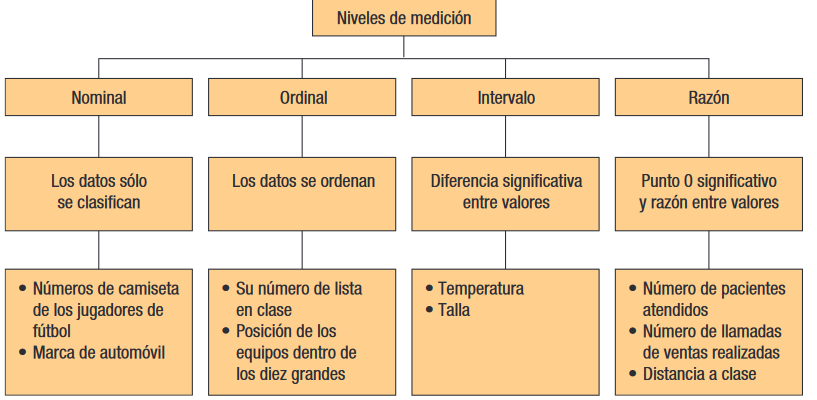
\includegraphics[width=16cm, height=8cm]{resumenCaracteristicasNivelesMedicion1_3}
\section{Capitulo 2. Descripcion de datos: tablas de frecuencias, distribuciones de frecuencias y su representacion grafica.}
\subsection{Descripción de datos.}
{\large Tabla de frecuencias, distribuciones de frecuencias y su representación grafica.}
\subsection{Construcción de una tabla de frecuencias.}
La estadistica descriptiva se encarga de organizar datos con el fin de mostrar la distribucion general de estos y el lugar en donde tienden concentrarse, ademas de señalar valores de datos pocos usuales o extremos. El primer procedimiento que se emplea para organizar y resumir un conjunto de datos es una \textbf{tabla de frecuencias.}
\begin{center}
	\textbf{Tabla de frecuencias:} Agrupacion de datos cualitativos en clases mutuamente excluyentes que muestra el numero de observaciones en cada clase.
\end{center}
Recordar que, una variable cualitativa es de naturaleza no numerica; es decir, que la informacion es clasificable en distintas categorias. No hay un order particular en estas categorias. Por otro lado, estan las variables cuantitativas son de indole numerica.
\subsubsection*{Frecuencias relativas de clase.}
Es posible convertir las frecuencias de clase en frecuencias relativas de clase para mostrar la fraccion del numero total de observaciones en cada una de ellas. Una frecuencia relativa capta la relacion entre la totalidad de elementos de una clase y el numero total de observaciones. Para convertir una distribucion de frecuencias en una distribucion de frecuencias relativa, cada una de las frecuencias de clase se divide entre el total de observaciones.

\subsubsection*{Representación grafica de datos cualitativos.}
El instrumento mas comun para representar una variable cualitativa en forma grafica es la \textbf{grafica de barras}. En la mayoria de los casos, el eje horizontal muestra la variable de interes y el eje vertical la frecuencia o fraccion de cada uno de los posibles resultados. Una caracteristica distinta de esta herramienta es que existe una distancia o espacio entre las barras. Una grafica de barras es una representacion grafica de una tabla de frecuencias mediante una serie de rectangulos de anchura uniforme, cuya altura corresponde a la frecuencia de clase.
\begin{center}
	\textbf{Grafica de barras:} En ella, las clases se representan en el eje horizontal y la frecuencia de clase en el eje vertical. Las frecuencias de clase son proporcionales a las alturas de las barras.
\end{center}
Se muestra ejemplo de una grafica de barras en la siguiente pagina:\\
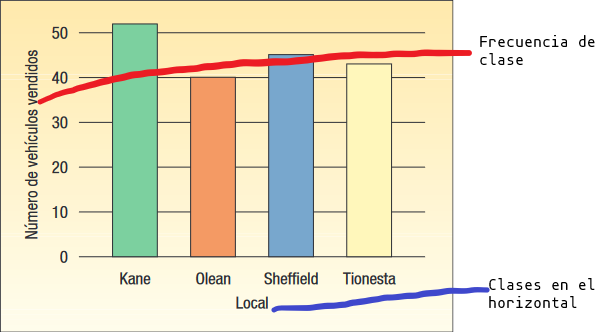
\includegraphics[width=13cm]{graficaBarras2_1.png} \\
Otro tipo de grafica util para describir informacion cualitativa es la \textbf{grafica de pastel}.
\begin{center}
	\textbf{Grafica de pastel: }Grafica que muestra la parte o porcentaje que representa cada clase del total de numeros de frecuencia.
\end{center}
El primer paso para elaborar una grafica de pastel consiste en registrar los porcentajes 0, 5, 10, 15, etc, de manera uniforme alrededor de la circunferencia de un circulo. El area rebanada representa alguna clase, cada rebanada de pastel representa la  porcion relativa de cada componente, es posible compararlas con facilidad.\\
Aca un ejemplo de grafica bizcochuelo.\\
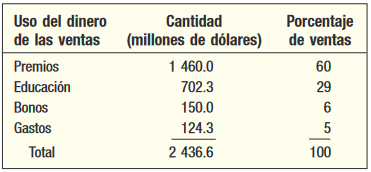
\includegraphics{tablaFrecuenciasRelativas2_2.PNG}\\
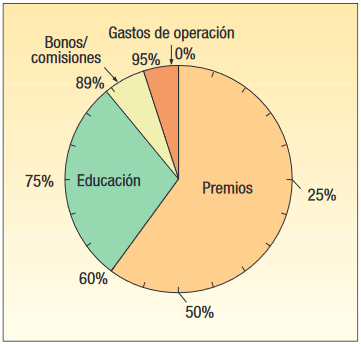
\includegraphics[width=12cm, height=10cm]{graficoPastel2_2.png} \\
Las graficas de pastel y las de barras cumplen casi la misma funcion. ¿Cuales son los criterios para elegir una u otra? En la mayoria de los casos, las graficas de pastel son las mas informativas cuando se trata de comparar la diferencia relativa en el porcentaje de observaciones de cada uno de las variables de la escala nominal. Es preferible usar una grafica de barras cuando el objetivo es comparar el numero de observaciones en cada categoria.
\subsection{Construcción de distribuciones de frecuencias: datos cuantitativos.}
Distribucion de frecuencias puede ser util para describir la ganancias de ventas.
\begin{center}
	\textbf{Distribucion de frecuencias: }Agrupacion de datos en clases mutuamente excluyentes, que muestra el numero de observaciones que hay en cada clase.
\end{center}
¿Como crear una distribucion de frecuencias? El primer paso consiste en acomodar los datos en una tabla que muestre las clases y el numero de observaciones que hay en cada clase. Recorda que el \textbf{objetivo} es construir tablas, diagramas y graficas que revelen rapidamente la concentracion, los valores extremos y la distribucion de los datos.
La informacion desorganizada como \textbf{datos en bruto} o \textbf{datos no agrupados}. Los datos en bruto se interpretan con mayor facilidad si se organizan como una distribucion de frecuencias.\\
\textbf{Paso 1: Defina el numero de clases.} El objetivo consiste en emplear suficientes agrupamientos o \textbf{clases}, de manera tal que se perciba la forma de la distribucion. Aca se necesita criterio. Una gran cantidad de clases o muy pocas podrian no permitir ver la conformacion fundamental del conjunto datos. Una receta util para determinar la cantidad de clases $(k)$ es la regla de 2 a la $k$. Esta guia sugiere que se elija el menor numero $ (k) $ para el numero clases, de tal manera que $ 2^{k} $ sea mayor que el numero de observaciones $ (n) $. Ejemplo $ n=180 $ obsevaciones, si supone $ k=7 $, lo cual significa que utilizara siete clases, entonces $ 2^{7}=128 $, algo menos que las 180 observaciones. De ahi que 7 no represente suficientes clases. Si $ k=8 $, entonces $ 2^{8}=256$, que es mayor 180. Por lo tanto, el numero de clases se recomienda es de 8. \\\\
\textbf{Paso 2: Determine el intervalo o ancho de clase.} El \textbf{intervalo} o \textbf{ancho de clase} deberia ser el mismo para todas las clases. Todas las clases juntas deben cubrir por lo menos la distancia del valor mas bajo al mas alto de los datos. Expresado esto en una formula seria:
\[ i\geq \frac{H-L}{k} \]
Por lo general el tamaño de intervalo se redondea a una cifra conveniente, tal como un multiplo de 10 a 100. En las distribuciones de frecuencia son preferibles los intervalos de clase iguales. Sin embargo, en ciertos casos se necesita que no lo sean para evitar una gran cantidad de clases vacias, o casi vacias.\\\\

\textbf{Paso 3: Establezca los limites de cada clase.} Este paso es importante para que sea posible incluir cada observacion en una sola categoria. Esto significa que debe evitar la superposicion de limites de clase confusos. Por ejemplo, clases como \$1300 - \$1400 y \$1400 - \$1500 no deberian emplearse porque no resulta claro si el valor de \$1400 pertenece a la primera o a la segunda clases. Las clases como \$1300 - \$1400 y \$1500 - \$1600 se emplean con frecuencia, aunque tambien pueden resultar confusas si no se conviene en redondear todos los datos de \$1450 o por arriba de esta cantidad a la segunda clase y los datos por debajo de \$1400 a la primera clase. Al redondear el intervalo de clase hacia arriba con el fin de obtener un tamaño conveniente de clase, se cubre un rango mas amplio que el necesario. Una directriz consiste en convertir el limite inferir de la primera clase en un multiplo del intervalo de clase. A veces esto no es posible, pero el limite inferior por lo menos debe redondearse.\\\\
\textbf{Paso 4: Anote las veces que encuentre las observaciones en el intervalo en las clases.}  \textbf{PONER IMAGEN PASO 4}
\\\\\textbf{Paso 5: Cuente el numero de elementos de cada clase.}  El numero de elementos que hay en cada clase recibe el nombre de \textbf{frecuencia de clase.} Por ejemplo en numero de \$200 a \$600 hay 8 observaciones, y en la clase de \$600 a \$1000 hay 11 observaciones. Por lo tanto la frecuencia de clase de la primera es de 8, mientras que en la segunda es de 11. Hay un total de 180 observaciones o frecuencias en todo el conjunto de datos. asi que la suma de todas las frecuencias debe ser igual a 180. \textbf{PONER TABLA2-7}\\\\
Con frecuencia apareceran otros dos terminos: \textbf{punto medio de clase} e \textbf{intervalo de clase.} El punto medio, que se encuentra entre los limites inferiores de dos clases consecutivas, se calcula sumando los limites interiores de clases consecutivas y dividiendo el resultado entre dos. En caso de la imagen del paso 5, el limite de clase interior de la primera clase es de \$200 y el siguiente limite es de \$600. El punto medio de clase \$400, que se calcula mediante la operacion \[ \frac{\$600+\$200}{2} .\] El punto medio de \$400 representa mejor. Para determinar el intervalo de clase, se resta el limite inferior de la clase del limite inferior de la siguiente clase, es decir \[ \$600 -\$200 =400.\]Tambien se puede determinar el intervalo de clase calculando la diferencia entre puntos medios consecutivos. El punto medio de la primera clase des de \$400 y el punto medio de la segunda clase es de \$800. La diferencia es de \$400.
\subsection{Distribución de frecuencias relativas}
Si se requiere resumir las ventas del ultimo mes utilizando ganancia por venta; seria util describir la ganancia de venta por medio de una distribucion de frecuencias.
\begin{center}
	\textbf{Distribucion de frecuencias: }Agrupacion de datos en clases mutuamente excluyentes, que muestra el numero de observaciones que hay en cada clase.
\end{center}
¿Como crear una distribucion de frecuencias? El primer paso consiste en acomodar los datos en una tabla que muestre las clases y el numero de observaciones que hay en cada clase. El objetivo es construir tablas, diagramas y graficas que revelen rapidamente la concentracion, los valores extremos y la distribucion de los datos. La informacion desorganizada como \textbf{datos en bruto} o \textbf{datos no agrupados.} Los datos en bruto se interpretan con mayor facilidad si se organizan como una distribucion de frecuencias.\\\\
\textbf{Paso 1: Defina el numero de clases: }El objetivo consiste en emplear suficientes agrupamientos o \textbf{clases}, de manera tal que se perciba la forma de la distribucion. Se necesita criterio. Una gran cantidad de clases o muy pocas podrian no permitir ver la conformacion fundamental del conjunto de datos. Una receta util para determinar la cantidad de clases (k) es la regla de 2 a la k. Esta guia sugiere que se elija el menor numero (k) para el numero de clases, de tal manera que \[2^{k}\] sea mayor que el numero de observaciones (n). Si $ n=180 $, si supone que $ k=7 $, lo cual significa que utilizara siete clases, entonces \[ 2^{7}=128 \], algo menos de 180. De ahi que 7 no represente suficiente clases. Si $ k=8 $, entonces \[ 2^{8}=256 \], que es mayor a 180. Por lo tanto, el numero de clases que se recomienda es de 8.\\\\
\textbf{Paso 2: Determine el intervalo o ancho de clase:} El \textbf{intervalo o ancho de clase} deberia ser el mismo para todas las clases. Todas las clases juntas deben cubrir por lo menos la distancia del valor mas bajo al mas alto de los datos. Expresado esto en una formula seria: \[ i\geq\frac{H-L}{k} \] en la que la $ i $ es el intervalo de clase; H, el maximo valor observado; L, el minimo valor observado, y k, el numero de clases. En la practica, por lo general este tamaño de intervalo se redondea a una cifra conveniente, tal como un multiplo de 10 a 100. Las distribuciones de frecuencia son preferibles los intervalos de clase iguales. Ciertos casos se necesita que no lo sean para evitar una gran cantidad de clases vacias, o casi vacias. Facilita la compresion de la informacion.\\\\
\textbf{Paso 3: Establezca los limites de cada clase:} Este paso es importante para que esa posible incluir cada observacion en una sola categoria. Esto significa que debe evitar la superposicion de limites de clase confusos. Ponele tenes una clase 200-400 y otra de 400-600 ¿el 400 va incluido en la primera clase o en la segunda clase? ACLARA ESO O NO ENTIENDO NADAAAAA.\\\\
\textbf{Paso 4: Anote las observaciones en las clases:} Se da un ejemplo en la imagen siguiente \textbf{AGREGAR TABLA DEL PASO 4}\\\\
\textbf{Paso 5: Cuente el numero de elementos de cada clase:} El numero de elementos que hay en cada clase recibe el nombre \textbf{frecuencia de clase.} En la clase \$200 a \$600 hay 8 observaciones, y en la clase de \$600 a \$1000 hay 11 observaciones. Por lo tanto, la frecuencia de clase de la primera clase es de 8, mientras que en la segunda es de 11. Hay un total de 180 observaciones o frecuencias en todo el conjunto de datos. Asi que la suma de todas las frecuencias debe ser igual a 180. \textbf{PEGAR TABLA2-7}
Las ventajas de condesar los datos de forma mas entendible y organizada compensa por mucho este desventaja. \linebreak[2]
Con frecuencia apareceran otros dos terminos: \textbf{punto medio de clase e intervalo de clase}. El punto medio, que se encuentra los limites inferiores de dos clases consecutivos, se calcula sumando los limites inferiores de clases consecutivas y dividiendo el resultado entre dos. Para determinar el intervalo de clase, se resta el limite inferior de la clase del limite inferior de la siguiente clase.
\subsection{Distribucion de frecuencias relativas.}
Convertir frecuencias de clase en frecuencias relativas de clase, igual que con los datos cualitativos, con el fin de mostrar la fraccion del total de observaciones que hay en cada clase. Una distribucion de frecuencias relativas convierte la frecuencia en un porcentaje. Para convertir una distribucion de frecuencia en una distribucion de frecuencia relativa, cada una de las frecuencias de las clases se divide entre el numero total de observaciones. A continuacion dejo la tabla de como serian una frecuencia relativa. \textbf{PONER TABLA 2-8}
\subsection{Representacion grafica de una distribucion de frecuencias.}
Es frecuente que se necesite una vista rapida de las tendencias de las ventas, los precios de las acciones o costos de hospitalizacion. A menudo, estas tendencias se describen por medio de tablas y graficas. Tres herramientas que seran de utilidad para representar graficamente una distribucion de frecuencias son el histograma, el poligono de frecuencias y el poligono de frecuencias acumuladas.
\subsubsection*{Histograma}
Un histograma de una distribucion de frecuencias basadas en datos cuantittivos se asemeja mucho a la grafica de barras, que muestra la distribucion de datos cualitativos. Las clases se señalan en el eje horizontal y las frecuencias de clase en el eje vertical. Las frecuencias de clase se representan por medio de las alturas de las barras. Existe una importante diferencia como consecuencia de la naturaleza de los datos. Por lo general, los datos cuantitativos se miden con escalas continuas, no discretas. Por lo tanto, el eje horizontal representa todos los valores posibles y las barras se colocan de forma adyacente para que muestren la naturaleza continua de los datos.
\begin{center}
	\textbf{Histograma: }Grafica en la que las clases se señalan en el eje horizontal y las frecuencias de clase en el eje vertical. Las frecuencias de clase se representan por medio de las altura dde las barras, que se dibujan de manera adyacente.
\end{center}
Mostraremos un ejemplo a continuacion.
\subsubsection*{Poligono de frecuencias}
Un poligono de frecuencias tambien muestra la forma que tiene una distribucion y es similar a un histograma. Consiste en segmentos de recta que conectan los puntos que forman las intersecciones de los puntos medios de clase y frecuencias de clase. El punto medio de cada clase se indica en una escala en el eje X y las frecuencias de clase en el Y. Recorda que el punto medio de clase es el valor localizado en el centro de una clase y representa los valores tipicos de ella (limite superior - limite inferior). La frecuencia de clase es el numero de observaciones que hay en una clase particular. Para construir un poligono de frecuencias, hay que desplazarse horizontalmente sobre la grafica al punto medio, y en seguida de manera vertical, la frecuencia de clase, donde se coloca un punto. Los valores X y de Y de este punto reciben el nombre de \textit{coordenadas}. El proceso cotinua con todas las clases. Posteriormente, los puntos se conectan de manera ordenada. Es decir, que el punto que representa la clase mas baja se une al que representa la segunda clase y asi en lo sucesivo. \textbf{PONER GRAFICA 2-5}\linebreak Tanto el histograma como el poligono de frecuencias permiten tener una vista rapida de las principales caracteristicas de los datos (maximos, minimos, puntos de concentracion, etc.). Aunque las dos representaciones tienen un proposito similar, el histograma posee la ventaja de que describe cada clase como un rectangulo, en el que la barra de altura de este representa el numero de elementos que hay en cada clase. El poligono de frecuencias, en cambio, tiene una ventaja con respecto al histograma. Tambien permite comparar directamente dos o mas distribuciones de frecuencias \textbf{PONER GRAFICA 2-6 DE EJEMPLO}.
\subsubsection*{Distribuciones de frecuencia acumulativas}.
Una distribucion de frecuencias acumulativas muestra el numero o porcentaje de observaciones por debajo de valores dados, con representacion grafica de un \textbf{poligono de frecuencias acumulativas.} Como su nombre lo indica, una distribucion de frecuencias acumulativas y un poligono de frecuencias acumulativas implican \textit{frecuencias acumulativas}. La frecuencia acumulativa basicamente vas sumando todas las frecuencias de las clases. \textbf{PONER TABLA 2-9}
Para trazar una distribucion de frecuencias acumulativas, \textbf{se ubica el limite superior de cada clase en una escala a lo largo del eje X}, y \textbf{las correspondientes frecuencias acumulativas, a lo largo del eje Y}. Para incluir informacion adicional, gradue el eje vertical a la izquierda en unidades y el eje vertical a la derecha en porcentajes.
\section{Capitulo 3. Descripcion de datos: medidas numericas.}
\subsection{Introduccion}
En este capitulo se presentan dos formas numericas de describir datos cuantitativos: las \textbf{medidas de ubicacion} y las \textbf{medidas de dispersion.} A las medidas de ubicacion a menudo se les llama promedios. El proposito de una medida de ubicacion consiste en señalar el centro de un conjunto devalores. Vos ya estas conoces el concepto de promedio (media aritmetica), medida de ubicacion que muestra el valor central de los datos. Si solo tomas las medidas de ubicacion en cuenta de un conjunto de datos o si compara varios conjuntos de datos utilizando valores centrales, llegara a una conclusion incorrecta. Ademas de las medidas de ubicacion, debe tomar en consideracion la \textbf{dispersion} (con frecuencia se le llama \textit{frecuencia variacion }o \textit{propagacion}) de los datos. Para describir la dispersion considere el rango, la desviacion media, la varianza y la desviacion estandar. En principio se explican las medidas de ubicacion. No existe una unica medida de dispersion; de hecho existen varias. Consideraremos cinco:
\begin{enumerate}
	\item La media aritmetica.
	\item La media ponderada.
	\item La mediana.
	\item La moda.
	\item La media geometrica.
\end{enumerate}
La medida aritmetica es la medida de ubicacion que mas se utiliza y que se publica con mayor frecuencia, por lo cual se le considerará como parametro para una poblacion y como estadistico para las muestras.
\subsection{La media poblacional}
La media poblacional es la suma de todos los valores observados en la poblacion dividida entre el numero de valores de la poblacion. Para determinar la media poblacional, aplique la siguiente formula con simbolos matematicos:
\[ \mu=\frac{\sum X}{N} \] 
En la cual:
\begin{enumerate}
	\item $\mu$ representa la media poblacional; se trata de la letra minuscula griega mu.
	\item $N$ es la numera de valores en la poblacion.
	\item $X$ representa cualquier valor particular.
	\item $\sum$ es la letra mayuscula griega sigma e indica la operacion de suma.
	\item $\sum X$ es la suma de X valores en la poblacion.
\end{enumerate}
\end{document}
